\documentclass[tikz,border=8pt]{standalone}
\usepackage{amsmath,amssymb}
\usetikzlibrary{arrows.meta,automata,positioning,quotes}
\begin{document}
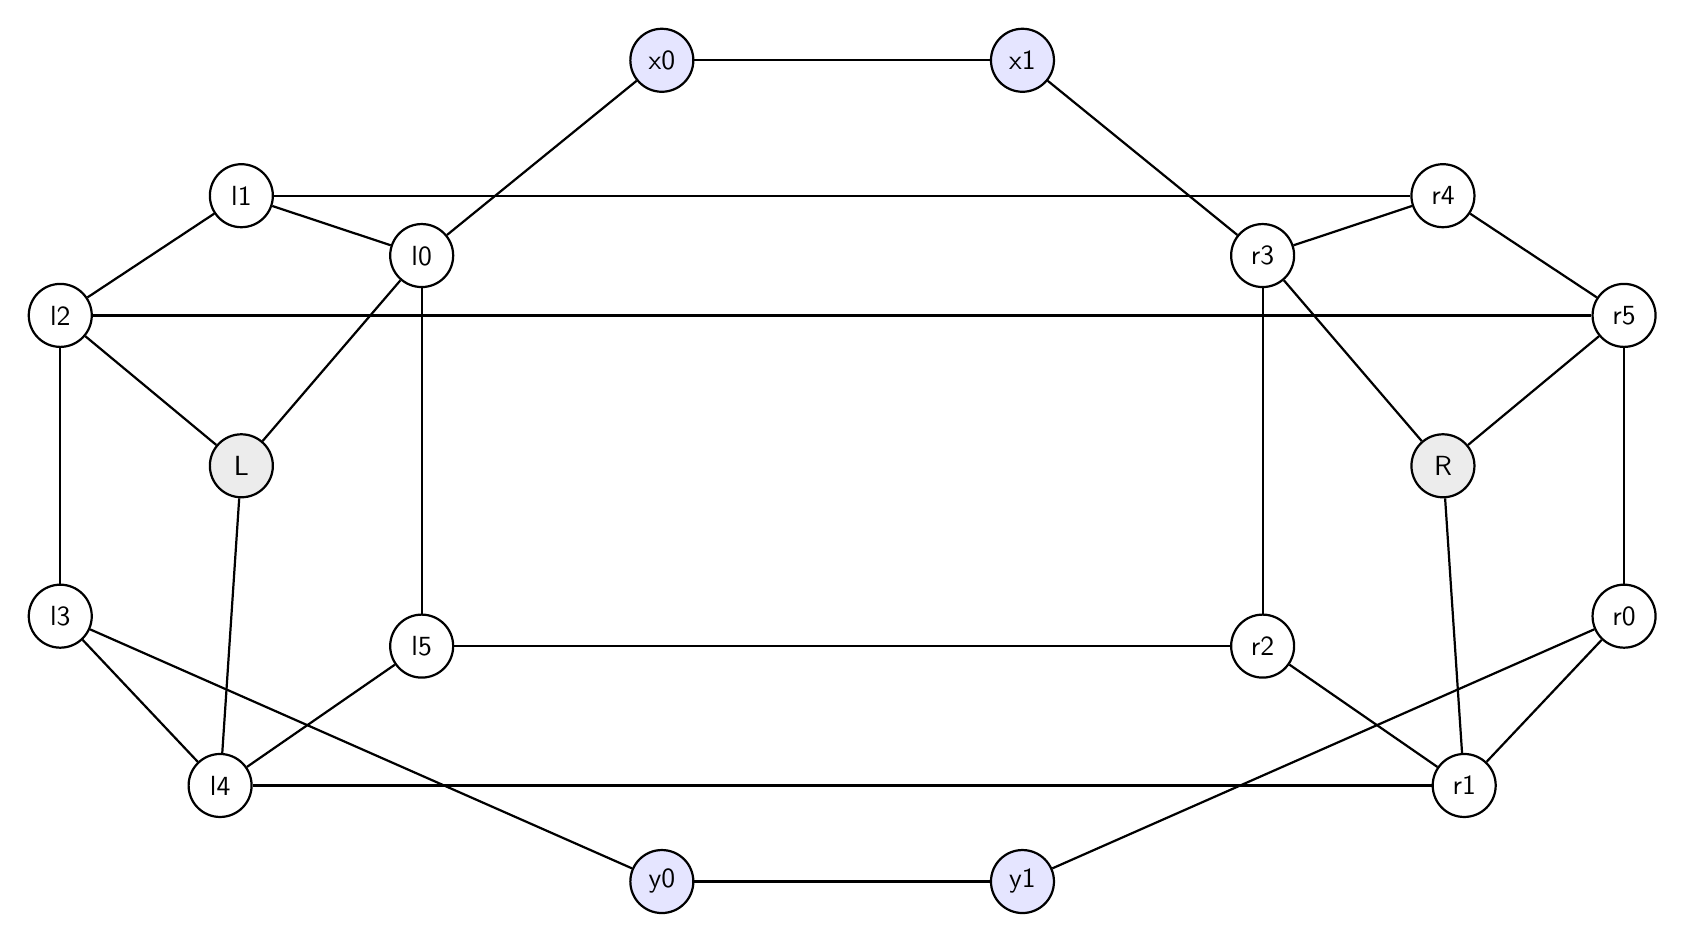
\begin{tikzpicture}[x=1cm,y=1cm]
\tikzset{
  graphnode/.style={circle,draw,thick,minimum size=8mm,inner sep=1pt,font=\sffamily},
  directed/.style={-{Stealth[length=2.4mm]},thick},
  undirected/.style={thick}
}
\node[graphnode,fill=gray!15] (n_L) at (-7.63,0.02) {L};
\node[graphnode] (n_l0) at (-5.34,2.69) {l0};
\node[graphnode] (n_l1) at (-7.63,3.45) {l1};
\node[graphnode] (n_l2) at (-9.93,1.93) {l2};
\node[graphnode] (n_l3) at (-9.93,-1.89) {l3};
\node[graphnode] (n_l4) at (-7.90,-4.04) {l4};
\node[graphnode] (n_l5) at (-5.34,-2.27) {l5};
\node[graphnode,fill=gray!15] (n_R) at (7.63,0.02) {R};
\node[graphnode] (n_r0) at (9.93,-1.89) {r0};
\node[graphnode] (n_r1) at (7.90,-4.04) {r1};
\node[graphnode] (n_r2) at (5.34,-2.27) {r2};
\node[graphnode] (n_r3) at (5.34,2.69) {r3};
\node[graphnode] (n_r4) at (7.63,3.45) {r4};
\node[graphnode] (n_r5) at (9.93,1.93) {r5};
\node[graphnode,fill=blue!10] (n_x0) at (-2.29,5.17) {x0};
\node[graphnode,fill=blue!10] (n_x1) at (2.29,5.17) {x1};
\node[graphnode,fill=blue!10] (n_y0) at (-2.29,-5.26) {y0};
\node[graphnode,fill=blue!10] (n_y1) at (2.29,-5.26) {y1};
\draw[undirected] (n_l0) -- (n_l1);
\draw[undirected] (n_l1) -- (n_l2);
\draw[undirected] (n_l2) -- (n_l3);
\draw[undirected] (n_l3) -- (n_l4);
\draw[undirected] (n_l4) -- (n_l5);
\draw[undirected] (n_l5) -- (n_l0);
\draw[undirected] (n_L) -- (n_l0);
\draw[undirected] (n_L) -- (n_l2);
\draw[undirected] (n_L) -- (n_l4);
\draw[undirected] (n_r0) -- (n_r1);
\draw[undirected] (n_r1) -- (n_r2);
\draw[undirected] (n_r2) -- (n_r3);
\draw[undirected] (n_r3) -- (n_r4);
\draw[undirected] (n_r4) -- (n_r5);
\draw[undirected] (n_r5) -- (n_r0);
\draw[undirected] (n_R) -- (n_r1);
\draw[undirected] (n_R) -- (n_r3);
\draw[undirected] (n_R) -- (n_r5);
\draw[undirected] (n_l0) -- (n_x0);
\draw[undirected] (n_x0) -- (n_x1);
\draw[undirected] (n_x1) -- (n_r3);
\draw[undirected] (n_l3) -- (n_y0);
\draw[undirected] (n_y0) -- (n_y1);
\draw[undirected] (n_y1) -- (n_r0);
\draw[undirected] (n_l1) -- (n_r4);
\draw[undirected] (n_l2) -- (n_r5);
\draw[undirected] (n_l4) -- (n_r1);
\draw[undirected] (n_l5) -- (n_r2);
\end{tikzpicture}
\end{document}
